\documentclass[a4paper]{article}

\usepackage{tikz}
\usepackage{graphicx}
%\usepackage{subfig}
\usepackage{algorithmicx}
\usepackage{float}
\usepackage{caption}
\usepackage{subcaption}
\usepackage{amsmath,amssymb,amsfonts, mathtools}
\usepackage{hyperref}
\usepackage{float}

\linespread{1.1}

\title{Descrete $p$-dispersion problem}
\author{Tilen Klinc, Janez Podlogar}
\date{\today}

\begin{document}
%%%%%%%%%%%%%%%%%%%%%%%%%%%%%%%%%%%%%%%%%%%%%%%%%%%%%%%%%%%%%%%%%%%%%
\maketitle
%%%%%%%%%%%%%%%%%%%%%%%%%%%%%%%%%%%%%%%%%%%%%%%%%%%%%%%%%%%%%%%%%%%%%

\section{Opis problema}

Obravnavamo problem izbire $ p $ točk iz nabora $ n $ točk v nekem prostoru
tako, da je minimalna razdalja med izbranimi točkami maksimizirana. Cilje je
izbrati točke tako, da so čim bolj ``razpršene''. Problem se pojavi v kontekstu
logistike, ko je bližina poslopji nezaželjena.


Za lokacije imamo podano lokacije $ I = \{ 1, 2, \ldots, n \} $ in matriko $ D \in 
\mathbb{R}^{n \times n} $, kjer nam $ d_{ij} \in D $ pove rezdaljo med lokacijo $ i $
in lokacijo $ j $. Brez škode za splošnost predpostavimo, da je matrika D simetrična in
da so njeni ne diagonalni elementi strogo pozitivni. Rešujemo optimizacijski problem
\begin{align*}
    & \max f(U) \\
    & \text{p.p. } f(U) = \min \{ d_{ij} \mid i,j \in U \text{ in } i \neq j \} \\
    & \qquad U \subseteq I \\
    & \qquad |U| = p .
\end{align*}

\section{Metode}

Za reševanje problema sva napisala tri algortime \textit{BruteForceMetoda}, \textit{PozresnaMetoda}
in \textit{BisekcijskaMetoda}.

\subsection{Izčrpna metoda}

Prva metoda je tako imenovana Brute Force in edina metoda, ki zagotavlja optimalno rešitev,
vendar je časovno neučinkovita. Generiramo vse možne nabore $ p $ točk izmed $ n $ točk in za vsak nabor
izračunamo najmanjšo razdaljo med izbranimi točkami. Med vsemi nabori točk izberemo
tistega, kjer je najmanjša razdalja med izbranimi točkami maksimizirana.

Ker je problem NP težak, metode nisva preizkušala na generiranih problemih, saj ima algoritem
eksponentno časovno zahtevnost.

\subsection{Požrešna metoda}

Požrešna metoda oziroma Greedy algoritem temelji na ideji, da na vsakem koraku izberemo
optimalno točko glede na prejšnji nabor točk. Za prvi dve točki izberemo najbolj oddaljeni
točki in ju dodamo v nabor. Naslednjo dodamo točko tako, da izberemo tisto točko, ki je med 
neizbranimi, od že izbranih točk, najbolj oddaljena. Postopek ponavljamo dokler ne izberemo 
$ p $ točk.

Metoda seveda ne nadje optimalne rešitve, vendar v zmernem času najde približek optimalne 
rešitve.

\subsection{Binarni linearni program z bisekcijo}

Problem reformuliramo na sledeč način.
Naj bo $ X = \{ x_i \mid 1 \leq i \leq n \} \text{ } $ vektor in matrika 
$ A(r) = \{ a_{ij}(r) \mid 1 \leq i < j \leq n \} $ tako, da velja 
\begin{align*}
	& x_i = 
	\begin{cases}
		1 \quad & \text{če \textbf{ne} izberemo }i\text{-te točke,} \\
		0 \quad & \text{sicer,}
	\end{cases}	\\
	& a_{ij}(r) =
	\begin{cases}
		0 \quad & \text{če } d_{ij} < r, \\
		1 \quad & \text{sicer.}
	\end{cases}
\end{align*}
Podan imamo naslednji matematični program
\begin{align}
    & \max r(p) \nonumber \\
    & \text{p.p. } x_i + x_j \geq a_{ij}(r) \qquad \text{za } 1 \leq i < j \leq 1 \label{eq1} \\
    & \qquad \textstyle\sum_{i=1}^{n}x_i = n - p \label{eq2} \\
    & \qquad x_i \in \{ 0,1 \} \,\;\qquad\qquad \text{za } 1 \leq i \leq 1 \label{eq3}.
\end{align}
Kriterijska funkcija $ r(p) $ je minimalna razdalja pri naboru $ p $ točk. Pogoj (\ref{eq2})
nam zagotovi, da izmed $ n $ točk izberemo natanko $ p $ točk. Nadalnje, pogoji (\ref{eq1}) nam zagotovijo,
da če sta točki oddaljeni za manj kot $ r $  izberemo kvečjemu eno. Torej ne bomo izbrali točk, ki bi bile med seboj
oddaljenje za manj kot $ r $. Bolj kot povečamo $ r $ bolj omejimo množico dopustnih točk. Iščemo torej maksimalni $ r $ 
pri katerem lahko še vedno izberemo $ p $ točk. Opomnimo, da desna stran pogojev (\ref{eq1}) ni fiksna, saj
je odvisna od $ r $, zato je program težko rešiti.

Formulacija nam narekuje , da poiščemo največjo $ r $ pri katerem je množica dopustnih rešitev natanko $ p $.
To naredimo na sledeč način. Če fiksirajmo $ r $ se problem imenujemo \textit{r-separation problem}. Iščemo najmanjše število
točk, ki so med seboj oddaljene vsaj za $ r $. Zapišemo sledeč linearni program
\begin{align*}
    & \min \textstyle\sum_{i=1}^{n}x_i \\
    & \text{p.p. } x_i + x_j \geq a_{ij}(r) \qquad \text{za } 1 \leq i < j \leq 1 \\
    & \qquad x_i \in \{ 0,1 \} \,\;\qquad\qquad \text{za } 1 \leq i \leq 1.
\end{align*}
Za algoritmični pristop k reševanju problema iz matrike $ D $ izluščimo vse razdalje med točkami in jih, z
upoštevajem večkratnosti, razporedimo po velikosti
\[
	r^1 \leq r^2 \leq r^3 \leq \cdots .
\]
Ker je $ r(p) $ nenaraščjoča funkcija argumenta $ p $ lahko poiščemo optimalni $ r^*(p) $ z \textit{line search}.
Očitno je, da je $ r^*(p) $ ena izmed razdalj $ r^k $. Pri iskanju se omejimo na njih. Prav tako lahko določimo
zgornjo mejo $ r^U $, kjer je $ U = \frac{1}{2}n(n-1) - \frac{1}{2}p(p-1) $. Določimo tudi trivialno
spodnjo mejo $ r^L $ pri $ L = n - p $. Sedaj po razdaljah
\[
	r^L \leq \cdots \leq r^U
\]
s pomočjo bisekcije poiščemo tak $ r^k $ pri katerejm je kriterijska funkcija enaka $ p $.
Če je kriterijska funkcija manjša od $ p $ se premaknemo na manjši $ r^k $ oziroma če, je 
manjša na večji $ r^k $.

\section{Generiranje primerov}

Za generiranje primerov sva napisala funkcijo \textit{GeneratorProblemov}. Funkcija 
sprejem argumetn $ n $, ki določi število naključno generiranih točk v ravnini, in 
vrne matriko $ D \in \mathbb{R}^{n \times n} $ razdalj med točkami. Drugi argument, ki ga prejme
je celo število $ p \in \{ 3, 4, 5 \ldots n \} $. Primeri, ko je $ p = 2 $ nas ne
zanimajo, saj so trivialno optimalno rešljivi.

\section{Testiranje modelov na generiranih podatkih}

Testirali smo dve metodi za reševanje problema. Prva metoda je bila bisekcijska metoda, druga pa požrešna metoda. Spreminjali smo tako $n$ kot $p$ parameter. Pri vsakem paru parametrov smo poskus ponovili za $100$ različnih problemov. Problem sestoji iz matrike razdalji, ki je velikosti $n \times n$ in parametra $p$, ki nam pove koliko lokacij si bomo izbrali. Matrike so bile naključno generirane, pri čemer smo upoštevali tudi trikotniško neenakost. Da je poskus ponovljiv smo tudi fiksirali random seed in sicer z $np.random.seed(2022)$. Ker se bisekcija metoda lahko zacikla, smo jo omejili, da se po $200$ ne uspelih poskusih samostojno prekine in vrne $None$, kar pomeni, da metoda ni skonvergirala.

\subsection{n = 10}
Najprej smo testirali pri $n = 10$. Ker imamo tukaj opravka še z razmeroma malimi matrikami, smo izvedli poskus za $p \in \{3, 4, 5, 6, 7\}$. Pri vsakem poskusu smo si zapisali najmanjšo razdaljo med točkami, par točk pri katerih je ta razdalja dosežena, množico vseh točk, ki jih imamo v izboru in čas izvajanja. Zanima nas predvsem katera metoda se je boljše odrezala. 

\begin{figure}[ht]
	\begin{subfigure}[t]{0.45\textwidth}
		\centering
		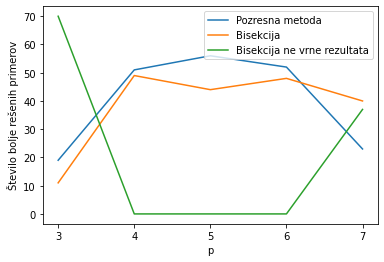
\includegraphics[width=\textwidth]{n_10.png}
		\caption{Uspešnost posamezne metode pri $n = 10$}
		\label{n_10_count}
	\end{subfigure}
	\hfill
	\begin{subfigure}[t]{0.45\textwidth}
		\centering
		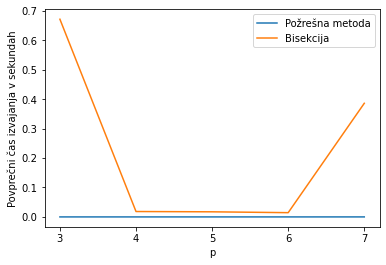
\includegraphics[width=\textwidth]{n_10_time.png}
		\caption{Povprečen čas izvajanja metode pri različnih $p$ in $n = 10$}
		\label{n_10_time}
	\end{subfigure}
    \caption{Rezultati pri $n = 10$.}
    \label{fig:n_10}
\end{figure}


Iz grafa je razvidno, da je bila bisekcija metoda pri $p = 3$ in $p = 7$ večkrat neuspešna in ni skonvergirala, medtem ko je pri $p \in \{4, 5, 6\}$ bila uspešna vsakič. 
Pri primerjavi dobljenih rezultatih je pri $p \in \{3, 4, 5, 6\}$ bila uspešnejša požrešna metoda, medtem ko se je to spremenilo pri $p = 7$, kjer je kljub neskonvergiranim vrednostim bila še vedno boljša bisekcijska metoda. 

Pogledali smo si tudi čas izvajanja posamezne metode. 

Vemo, da v primerih $p = 3$ in $p = 7$ metoda ni skonvergirala, torej je tam očitno čas izvajanja večji. Pri ostalih $p$ pa je čas izvajanja pri obeh metodah primerljiv.

\subsection{n = 20}
Nadalje smo testirali metodo pri $n = 20$. Poskus smo najprej ponovili za $p \in \{5, 10, 15\}$, ker pa sta metodi dobro konvergirali, smo dodali še dva parametra, tako da smo si pogledali pri $p \in \{5, 8, 10, 12, 15\}$. Tudi tukaj smo si pogledali, kako uspešna je posamezna metoda. 

\begin{figure}[ht]
	\begin{subfigure}[t]{0.45\textwidth}
		\centering
		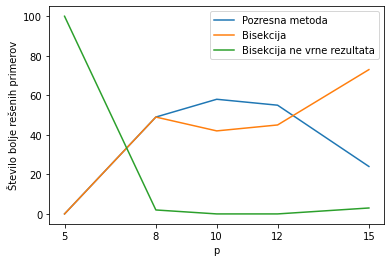
\includegraphics[width=\textwidth]{n_20.png}
		\caption{Uspešnost posamezne metode pri $n = 20$l}
		\label{n_20_count}
	\end{subfigure}
	\hfill
	\begin{subfigure}[t]{0.45\textwidth}
		\centering
		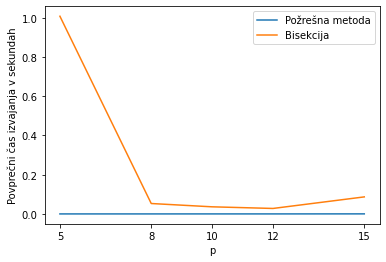
\includegraphics[width=\textwidth]{n_20_time.png}
		\caption{Povprečen čas izvajanja metode pri različnih $p$ in $n = 20$}
		\label{n_20_time}
	\end{subfigure}
    \caption{Rezultati pri $n = 20$.}
    \label{fig:n_20}
\end{figure}

Bisekcijska metoda spet ni skonvergirala za najmanjši $p$, je pa bila z večanjem $p$ čedalje bolj uspešna. Pri $p \in \{5, 8, 10, 12\}$ je spet prevladovala požrešna metoda, pri $p = 15$, pa se je za bistveno boljšo izkazala bisekcijska metoda, čeprav parkrat vseeno ni skonvergirala. 

Tudi v tem primeru ne moremo primerjati časa izvajanja metode pri najmanjšem $p = 5$, saj bisekcijska metoda tudi tukaj ni skonvergirala. Pri ostalih $p$ pa vidimo da je čas izvajanja spet primerljiv, pri čemer pa se za največji $p = 15$ začne čas že povečevati, je pa ta sprememba še vedno sprejemljiva.

\subsection{n = 50}
Nazadnje smo pogledali še $n = 50$. Tukaj smo si prav tako najprej zastavili $3$ parametre $p$ in sicer $p \in \{10, 25, 40\}$. Čas izvajanja je bil še sprejemljiv, tako da smo tudi tokrat povečali množico parametrov, tako da smo si ogledali za $p \in \{10, 20, 25, 30, 40\}$. 

\begin{figure}[H]
	\begin{subfigure}[t]{0.45\textwidth}
		\centering
		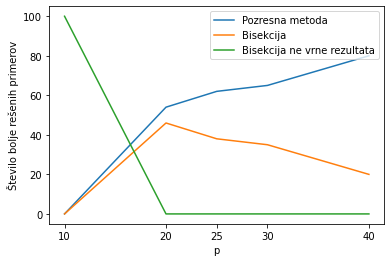
\includegraphics[width=\textwidth]{n_50.png}
		\caption{Uspešnost posamezne metode pri $n = 50$}
		\label{n_50_count}
	\end{subfigure}
	\hfill
	\begin{subfigure}[t]{0.45\textwidth}
		\centering
		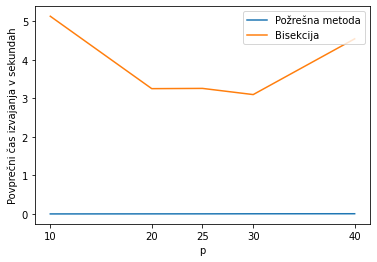
\includegraphics[width=\textwidth]{n_50_time.png}
		\caption{Povprečen čas izvajanja metode pri različnih $p$ in $n = 50$}
		\label{n_50_time}
	\end{subfigure}
    \caption{Rezultati pri $n = 50$.}
    \label{fig:n_50}
\end{figure}

Tako kot v prejšnjih primerih tudi tokrat bisekcijska metoda ni skonvergirala za najmanjši $p$. Se je pa v primerjavi s prejšnjimi primeri njena uspešnost tokrat slabšala. Požrešna metoda je bila tukaj za vse $p$ bolj uspešna.

Tudi z vidika časovne zahtevnosti, se je požrešna metoda izkazala za bistveno boljšo. Povprečni čas izvajanja z bisekcijsko metodo, je bil namreč za kar par sekund počasnejši kot čas izvajanja požrešne metode. Glede na rezultate bisekcije metode z počasnejšim in zahtevnejšim algoritmom nismo pridobili boljšega rezultata. 

\end{document}

